\section{Motivation}

We motivate the need to have a formal reasoning framework for weakly
isolated transactions through a series of simple examples that
abstract real-world scenarios.  All of our examples are written in a
C-like imperative language equipped with a \C{txn} lexical block
defining a transaction scope.  Each \C{txn} block is associated with
an identifier that uniquely identifies the transaction. We use Hoare
triple notation to annotate programs with pre- and post-conditions.

\begin{figure}
\centering
$\{\{\texttt{C}=\texttt{k} \conj \texttt{k}\ge\texttt{a1+a2}\}\}$
\begin{tabular}{l||l}
\begin{txnimpcode}
  txn '\B{Wd1}' {
    if (C $\ge$ a1) {
      C := C - a1
    }
  }
\end{txnimpcode}
&
\begin{txnimpcode}
  txn '\B{Wd2}'  {
    if (C $\ge$ a2) {
      C := C - a2
    }
  }
\end{txnimpcode}
\\
\end{tabular}
$\{\{\texttt{C}=\texttt{k-a1-a2}\}\}$

\caption{Concurrent withdraw transactions}
\label{fig:motiv-eg-1}
\end{figure}

Consider an implementation of a banking application that admits
concurrent withdraw transactions on a checking account (\C{C}), as
shown in Fig.~\ref{fig:motiv-eg-1}. If the initial balance (\C{k}) in
the account is enough to perform both withdraw operations, then the
final balance, after both transactions commit, is expected to reflect
the effects of performing these withdraws. The pre- and
post-conditions in Fig.~\ref{fig:motiv-eg-1} reflect our
expectations. Indeed, invariants are guaranteed to hold if both
withdraw transactions are serialized, making a \emph{serializable}
isolation ({\sc ser}) level a sufficent condition to preserve the
desired invaraint. But, is {\sc SER} necessary?

% Most weak isolation levels allow executions to interleave operations
% (Reads, Writes and Commits) of one transaction with other's, while
% enforcing some additional constraints. Arbitrary interleavings may
% lead to the violation of invaraints. 
As an alternative, consider the execution of this transaction under a
\emph{read committed} ({\sc rc}) isolation level, which is weaker than
     {\sc ser}\footnote{{\sc rc} is in fact the default isolation
       level in Postgres 9.5~\cite{postgres95} and Oracle
       11g~\cite{oracle11g} databases.} An {\sc rc} transaction is
     isolated from the writes of uncommitted transactions, thus
     preventing the transaction from witnessing \emph{dirty
       reads}~\cite{berenson}, reads that observe the effects of
     non-committed transactions.  In the current example, {\sc rc}
     isolation admits the two executions shown in Fig.~\ref{fig:rc-ex}.

\begin{figure}[!h]
\centering
\subcaptionbox {
  RC Execution 1
  \label{fig:motiv-eg-1-a}
} [
  0.55\columnwidth
] {
  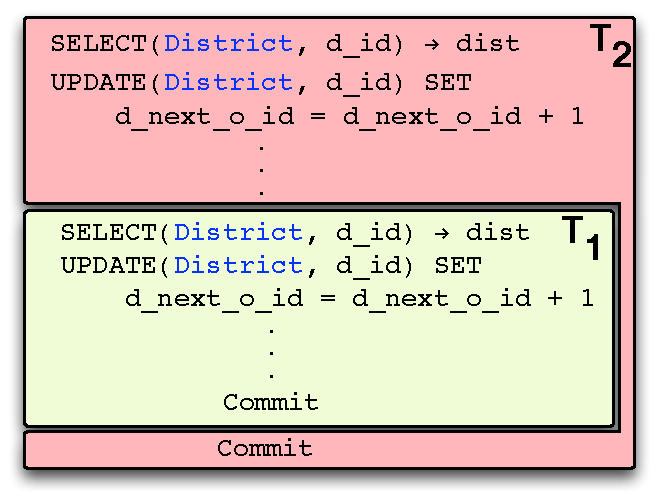
\includegraphics[scale=0.5]{Figures/motiv-eg-1-a}
}
%\hspace*{0.5in}
\subcaptionbox {
  RC Execution 2
  \label{fig:motiv-eg-1-b}
}{
  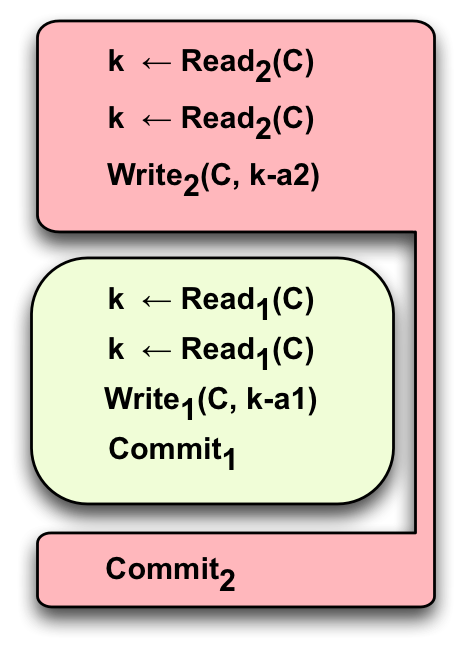
\includegraphics[scale=0.5]{Figures/motiv-eg-1-b}
}
\caption{Two possible executions under an {\sc rc} isolation level.}\label{fig:rc-ex}
\end{figure}

The figure depicts an execution as a series of read, write, and commit
operations.  The subscript of an operation indicates the transaction
that executes it\footnote{For clarity, the effects of different
  transactions are shown in different colored backgrounds.} In the
first execution, transaction {\bf Wd1} reads the current balance
(\C{k}) and writes the new balance (\C{k-a1}), but before it commits
transaction {\bf Wd2} executes and commits, writing the new balance
(\C{k-a2}). RC isolation prevent {\bf Wd2} from witnessing the
uncommitted writes of transaction {\bf Wd1}.  Subsequently committing
{\bf Wd1} leads to the loss of {\bf Wd2}'s updates (the so called
\emph{lost update anomaly}~\cite{berenson}), resulting in an incorrect
balance of \C{k-a1}. The second execution describes a similar scenario
with {\bf Wd1} and {\bf Wd2} exchanging their roles.

Clearly, using a \emph{read committed} isolation level is not
sufficient because it may result in the loss of updates from one
transaction and can thus violate the invariant given in
Fig.~\ref{fig:motiv-eg-1}. Now, consider an alternative unfolding of
Execution 1, where, rather than committing {\bf Wd1} and overwriting
the updates of {\bf Wd2}, we rollback {\bf Wd1} to reexecute it
starting from the state that contains the updates of {\bf Wd2}. No
updates are lost in this alternative execution, leading to the
satisfaction of Fig.~\ref{fig:motiv-eg-1}'s invariant. Rolling back
and reexecuting an uncommitted transaction to prevent write-write
conflicts with a committed transaction is a strategy often adopted by
databases that implement \emph{snapshot isolation} ({\sc si}). Indeed,
{\sc si} is sufficient to enforce the required invariants in this
example\footnote{\emph{Parallel snapshot isolation} ({\sc psi}), a
  weaker version of {\sc si} tailor-made for replicated stores is also
  sufficient.}.  Moreover, relying on optimistic speculation instead
of pessimistic locking for concurrency control enables {\sc si} to
often be more efficient than {\sc ser}, making it appropriate for the
transactions shown in Fig.~\ref{fig:motiv-eg-1}.  Note that we have
arrived at the applicability of {\sc si} (and the inapplicability of {\sc
  rc}) via a number of \emph{ad hoc} reasoning steps, several of which
are based on speculation about a the underlying data store's
implementation strategies. Such a reasoning process is necessarily
fragile and error-prone. 

\begin{figure}
\centering
$\{\{\texttt{C+S}\ge\texttt{0}\}\}$
\begin{tabular}{l||l}
\begin{txnimpcode}
  txn '\B{WdC}' {
    if (C+S $\ge$ a1) {
      C := C - a1
    }
  }
\end{txnimpcode}
&
\begin{txnimpcode}
  txn '\B{WdS}' {
    if (C+S $\ge$ a2) {
      S := S - a2
    }
  }
\end{txnimpcode}
\\
\end{tabular}
$\{\{\texttt{C+S}\ge\texttt{0}\}\}$

\caption{Withdraws from current (\C{C}) and savings (\C{S}) accounts.}
\label{fig:motiv-eg-2}
\end{figure}

{\sc si} effectively serializes updates to a data object without
relying on expensive lock-based concurrency control. While this makes
it a better alternative to {\sc ser} in some cases, it cannot however
serve as a replacement for the latter. Consider a different banking
application that maintains a current (\C{C}) and savings account
(\C{S}) for each user. A user can withdraw either from current or from
savings as long as the combined balance is at least as much as the
amount being withdrawn.  Fig.~\ref{fig:motiv-eg-2} shows a pair of
concurrent transactions, {\bf WdC} and {\bf WdS}, performing
withdrawls from current and savings accounts, resp. The pre-
and post-conditions for this program assert that executing its
transactions will not result in a non-negative combined balance.  {\sc
  ser} is sufficient to preserve the invariant, but {\sc si} is not.
Intuitively, this is because there are no \emph{lost updates} in this
example even when both transactions commit concurrently, hence there
is no reason for {\sc si} to serialize them. A reasoning framework for
weak isolation should let us formally deduce this fact by making it
impossible to construct a proof of correctness for the program under
{\sc si}, but facilitating a proof under {\sc ser}.

\begin{figure}[t]
\centering
$\{\{\texttt{C+S}\ge\texttt{0}\}\}$
\begin{tabular}{l||l||}
\begin{txnimpcode}
  txn '\B{Xfer}' {
    C := C - a;
    S := S + a;
  }
\end{txnimpcode}
&
\begin{txnimpcode}
  txn '\B{TotBal}' {
    T := S + C
  }
\end{txnimpcode}
% \\
% \multicolumn{2}{c} {
% }
\end{tabular}
\begin{tabular}{c}
  \begin{txnimpcode}
    txn '\B{AddInt}' {
      S := S + (T*0.1)
    }
  \end{txnimpcode}
\end{tabular}

$\{\{\texttt{C+S}\ge\texttt{0}\}\}$

\caption{Concurrent transfer (\C{Xf}) and interest accumulation (\C{Int}).}
\label{fig:motiv-eg-3}
\end{figure}

The previous example preserves invariants on \C{C} and \C{S} by
effectively serializing those transactions that write to \C{C} and
\C{S}.  However, in general, serializing a subset of transactions that
write to the data objects referenced by invariants is neither
necessary nor sufficient to ensure desired invariants hold. Consider
the banking application in Fig.~\ref{fig:motiv-eg-3} with three
transactions. Transaction {\bf Xfer} transfers some amount (\C{a})
from the current (\C{C}) to the savings (\C{S}) account.  Transaction
{\bf TotBal} records the total balance in both accounts in a data
object \C{T}, and transaction {\bf AddIntr} calculates interest on the
total balance (10\% of \C{T}) and adds it to the savings
account. Using a data object to record some function of the current
state of other data objects is a standard practice in relational
databases, where materialized views~\cite{oraclematview} are created
to maintain the results of a SQL query. Like the previous example, the
invariant of interest in this example is a non-negative total balance.
However, unlike the previous example, serializing transactions that
write to \C{C} and \C{S} is not sufficient to guarantee the invariant.
The execution shown in Fig.~\ref{fig:motiv-eg-3-a} demonstrates this anomaly:

\begin{figure}[!h]
\centering
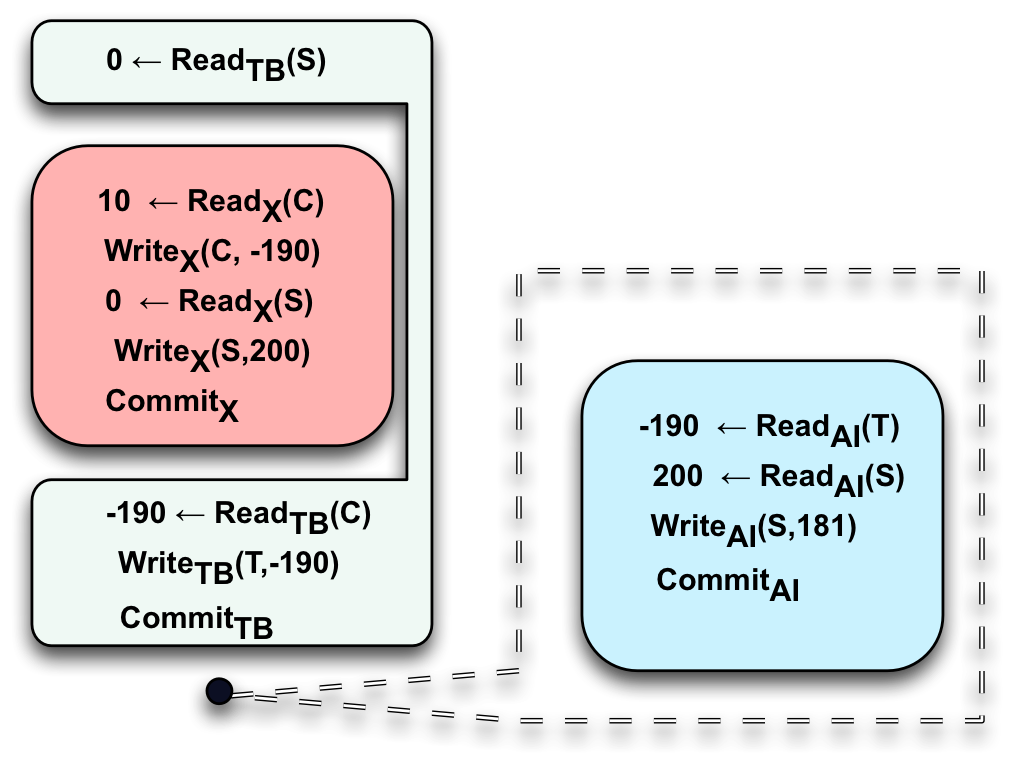
\includegraphics[scale=0.5]{Figures/motiv-eg-3-a}
\caption{Serializing transactions that update objects referenced by
  program invariants may introduce unwanted anomalies.}
\label{fig:motiv-eg-3-a}
\end{figure}

The subscripts {\bf X}, {\bf TB} and {\bf AI} denote {\bf Xfer}, {\bf
  TotBal} and {\bf AddInt} transactions, resp. Assume that \C{C} and
\C{S} are initially 10 and 0, resp.  Assume \C{a} is 200, i.e., we
subtract 200 from \C{C} and add it to \C{S}.  Transferring amounts
from \C{C} to \C{S} is allowed because the total balance invariant is
not affected.  The execution begins with {\bf TotBal} transaction
reading the savings (\C{S}) balance as 0 (we assume left-to-right
evaluation order for \C{S + C}).  However, before it reads the current
(\C{C}) balance, the {\bf Xfer} transaction executes and commits,
changing \C{C} to -190.  Subsequently, {\bf TotBal} reads -190 from
\C{C}, and updates \C{T} to -190. {\bf AddInt}, which begins execution
after {\bf TotBal}, reads -190 from \C{T}, calculates the interest as
-19, and updates \C{S} to 181. The result is a state with a total
balance of -9, a value that violates the invariant.

Note that transactions {\bf Xfer} and {\bf AddInt}, which write to the
data objects (\C{C} and \C{S}) relevant to the invariant, are
serialized in the above execution. Transaction {\bf TotBal}, however,
is not.  Although serializing it would fix the problem, it is not
necessary. A simpler fix would be to isolate {\bf TotBal} transaction
from the effects of a concurrent executing {\bf Xfer} transaction, so
that it reads \C{C} as 10 despite {\bf Xfer} committing -190 to
\C{C}. This can be achieved by executing {\bf TotBal} under a
\emph{repeatable read} ({\sc rr}) isolation level, which guarantees
that any two reads of a data object in a transaction return the same
value.  Allowing {\bf Xfer} to interfere with {\bf TotBal} violates
the repeatable read property since a hypothetical read from \C{S} in
{\bf TotBal} after the interference returns a different value (200)
than the first read (0). Executing {\bf TotBal} under {\sc rr}
effectively prohibits such interference.

\begin{figure}[t]
\centering
\hspace*{-0.3in}$\{\{\texttt{V=0}\}\}$
\begin{tabular}{l||l}
\begin{txnimpcode}
  txn '\B{Rd}' {
    X := V
    Y := V
  }
\end{txnimpcode}
&
\begin{txnimpcode}
  cobegin (i $\leftarrow$ [1$\ldots$3]) {
    txn '\B{Inc}$_{i}$' {
      V := V + 1
    }
  }
\end{txnimpcode}
% &
% \begin{txnimpcode}
%   txn$\langle$'Inc2'$\rangle${
%     V := V + 1
%   }
% \end{txnimpcode}
\\
\end{tabular}
\hspace*{-0.3in}$\{\{\texttt{Y}\ge\texttt{X}\}\}$

\caption{View counter (\C{V}) increments (\C{Inc}) and reads (\C{Rd})}
\label{fig:motiv-eg-4}
\end{figure}

%% SJ: not sure this example is needed - seems very complex, and introduces
%% details about the weak consistency.
Our last example demonstrates that it is not necessary to serialize
transactions, even if they write to the same data objects, to maintain
essential invariants in practical applications. Consider a counter
used to count video views on a YouTube-like application. The counter
need not accurately track the view count, but it must at least ensure
that the count does not decrease (nor does it appear to be
decreasing). Fig.~\ref{fig:motiv-eg-4} shows a simple example
involving a view counter (\C{V}). The three {\bf Inc} transactions
({\bf Inc$_{1}$}, {\bf Inc$_{2}$}, and {\bf Inc$_{3}$}) increment the counter,
while {\bf Rd} transaction reads the counter twice and writes the
values read to \C{X} and \C{Y}, resp. The count is 0 initially. Since
we expect the view count to monotonically increase, we require
$\C{Y}\ge\C{X}$ after all transactions commit.  Under a sequentially
consistent setting, where new writes to data objects always overwrite
previous writes, executing the increment transactions under a weak
isolation level can violate the monotonicity invariant, by allowing a
transaction to read a stale value for \C{V}, a value that has already
been updated by another.


%% the post-condition may not hold. For instance,
%% consider an execution where `{\bf Inc[1]}' reads \C{V} as 0 (but doesn't
%% commit), then `{\bf Inc[2]}' and `Inc[3]' commit serially changing \C{V} to
%% 2, followed by `Rd' reading 2 and writing it to \C{X}. Now `Inc[1]',
%% which has read \C{V} as 0 writes 1 to \C{V} and commits. The
%% subsequent read of \C{V} by `Rd' returns 1, which it writes to \C{Y}
%% and commits. In the final state, \C{X} is 2 and \C{Y} is 1, thus
%% violating the monotonicity invariant.

However, when executed in a weakly consistent environment, such as
those found in modern day replicated data stores, writes arriving at a
replica need not necessarily overwrite existing writes. A
\emph{conflict resolution strategy} may be employed to pick, for
example, a write with the largest value among competing concurrent
writes. Under this setting, the write to \C{V} by {\bf Inc$_{1}$} with a
value less than the current value is discarded. Transaction
{\bf Rd} therefore continues to read a value consistent with the invariant, allowing it to satisfy the
post-condition. Note that we did not have to serialize any of the {\bf Inc}
transactions to uphold the invariant, although they are
all involved in write-write conflicts.  A \emph{read committed}
isolation level suffices\footnote{We have implicitly assumed that `Rd'
  transaction witnesses monotonically growing state, i.e., the
  transactions that appear committed to the first read of \C{V} in
  `Rd' also appear committed to the second read.  Most implementations
  of RC enforce this \emph{Monotonic View} invariant. However,
  some~\cite{pldi15,bailishat} categorize {\sc rc} with \emph{monotonic view} as a
  separate isolation level called \emph{monotonic atomic view}
  ({\sc mav}). On those stores, we need {\bf Rd} to execute under {\sc mav} isolation.}, provided that the
conflict resolution strategy consistently picks writes with larger
values. A reasoning framework for weak isolation must be sensitive to
the semantics of conflict resolution in order to formally prove the
monotonicity invariant in this example.

